\documentclass{sigchi}

% Use this command to override the default ACM copyright statement
% (e.g. for preprints).  Consult the conference website for the
% camera-ready copyright statement.

%% EXAMPLE BEGIN -- HOW TO OVERRIDE THE DEFAULT COPYRIGHT STRIP -- (July 22, 2013 - Paul Baumann)
% \toappear{Permission to make digital or hard copies of all or part of this work for personal or classroom use is      granted without fee provided that copies are not made or distributed for profit or commercial advantage and that copies bear this notice and the full citation on the first page. Copyrights for components of this work owned by others than ACM must be honored. Abstracting with credit is permitted. To copy otherwise, or republish, to post on servers or to redistribute to lists, requires prior specific permission and/or a fee. Request permissions from permissions@acm.org. \\
% {\emph{CHI'14}}, April 26--May 1, 2014, Toronto, Canada. \\
% Copyright \copyright~2014 ACM ISBN/14/04...\$15.00. \\
% DOI string from ACM form confirmation}
%% EXAMPLE END -- HOW TO OVERRIDE THE DEFAULT COPYRIGHT STRIP -- (July 22, 2013 - Paul Baumann)

% Arabic page numbers for submission.  Remove this line to eliminate
% page numbers for the camera ready copy
% \pagenumbering{arabic}

% Load basic packages
\usepackage{balance}  % to better equalize the last page
\usepackage{graphics} % for EPS, load graphicx instead 
\usepackage[T1]{fontenc}
\usepackage{txfonts}
\usepackage{mathptmx}
\usepackage[pdftex]{hyperref}
\usepackage{color}
\usepackage{booktabs}
\usepackage{textcomp}
% Some optional stuff you might like/need.
\usepackage{microtype} % Improved Tracking and Kerning
% \usepackage[all]{hypcap}  % Fixes bug in hyperref caption linking
\usepackage{ccicons}  % Cite your images correctly!
% \usepackage[utf8]{inputenc} % for a UTF8 editor only

% If you want to use todo notes, marginpars etc. during creation of your draft document, you
% have to enable the "chi_draft" option for the document class. To do this, change the very first
% line to: "\documentclass[chi_draft]{sigchi}". You can then place todo notes by using the "\todo{...}"
% command. Make sure to disable the draft option again before submitting your final document.
\usepackage{todonotes}

% Paper metadata (use plain text, for PDF inclusion and later
% re-using, if desired).  Use \emtpyauthor when submitting for review
% so you remain anonymous.
\def\plaintitle{SIGCHI Conference Proceedings Format}
\def\plainauthor{First Author, Second Author, Third Author,
  Fourth Author, Fifth Author, Sixth Author}
\def\emptyauthor{}
\def\plainkeywords{Authors' choice; of terms; separated; by
  semicolons; include commas, within terms only; required.}
\def\plaingeneralterms{Documentation, Standardization}

% llt: Define a global style for URLs, rather that the default one
\makeatletter
\def\url@leostyle{%
  \@ifundefined{selectfont}{
    \def\UrlFont{\sf}
  }{
    \def\UrlFont{\small\bf\ttfamily}
  }}
\makeatother
\urlstyle{leo}

% To make various LaTeX processors do the right thing with page size.
\def\pprw{8.5in}
\def\pprh{11in}
\special{papersize=\pprw,\pprh}
\setlength{\paperwidth}{\pprw}
\setlength{\paperheight}{\pprh}
\setlength{\pdfpagewidth}{\pprw}
\setlength{\pdfpageheight}{\pprh}

% Make sure hyperref comes last of your loaded packages, to give it a
% fighting chance of not being over-written, since its job is to
% redefine many LaTeX commands.
\definecolor{linkColor}{RGB}{6,125,233}
\hypersetup{%
  pdftitle={\plaintitle},
% Use \plainauthor for final version.
%  pdfauthor={\plainauthor},
  pdfauthor={\emptyauthor},
  pdfkeywords={\plainkeywords},
  bookmarksnumbered,
  pdfstartview={FitH},
  colorlinks,
  citecolor=black,
  filecolor=black,
  linkcolor=black,
  urlcolor=linkColor,
  breaklinks=true,
}

% create a shortcut to typeset table headings
% \newcommand\tabhead[1]{\small\textbf{#1}}

% End of preamble. Here it comes the document.
\begin{document}

\title{Project Report: Finite Elements Analysis for OsteoApp}

\numberofauthors{3}
\author{%
  \alignauthor{Baihan Lin\\
    \affaddr{UbiComp Lab}\\
    \affaddr{University of Washington}\\
    \affaddr{Seattle, WA 98105, USA}\\
    \email{doerlbh@gmail.com}}\\
}

\maketitle

\begin{abstract}
The project aims to conduct a finite element analysis (FEA) on a bone-like structure to simulate the vibration properties of a bone or arm. This simulation is supportive to OsteoApp, a smartphone app for personal osteoporosis screening that tests bone density and tells people if they are at risk for bone disease. OsteoApp uses a vibration technique that takes advantage of the accelerometers on a hand-held smartphone to measure bone stiffness and density, based on the vibrations that pass through the user's arm when the elbow is tapped. The FEA simulation in this study can help us better understand the relationship between the external tapping with the measured signals. This study is conducted by Baihan Lin, mentored by Morelle Arian and Josh Fromm, and supervised by Prof. Shwetak Patel.

\end{abstract}

\category{H.5.m.}{Information Interfaces and Presentation
 (e.g. HCI)}{Miscellaneous}{}{}

\keywords{signal processing, ubiquitous computing, health sensing, mobile phones, osteoporosis screening, finite elements analysis}

\section{Introduction}

The finite element analysis (FEA) on a bone-like structure to simulate the vibration properties of a bone or arm. This simulation is supportive to OsteoApp, a smartphone app for personal osteoporosis screening that tests bone density and tells people if they are at risk for bone disease. OsteoApp uses a vibration technique that takes advantage of the accelerometers on a hand-held smartphone to measure bone stiffness and density, based on the vibrations that pass through the user's arm when the elbow is tapped. The FEA simulation in this study can help us better understand the relationship between the external tapping with the measured signals.

\section{Progress} 

UPDATE-\today: Currently, I have constructed a 

\subsection{2017/03/30: Interview and Setup}

\subsection{2017/04/04: Decide on project}

\subsection{2017/04/11: Basic construction of model}

As shown in Figure~\ref{fig:figure1} from $Grey's$ $Anatomy$ \cite{WikipediaEN:Arm}, The humerus is the (upper) arm bone. It joins with the scapula above at the shoulder joint (or glenohumeral joint) and with the ulna and radius below at the elbow joint.

\begin{figure}
\centering
  \includegraphics[width=0.9\columnwidth]{figures/human_arm_bones_diagram}
  \caption{Bones of the upper limbs, together with shoulder girdles together comprising the human arm}~\label{fig:figure1}
\end{figure}


\begin{table}
  \centering
  \begin{tabular}{l r r r}
    % \toprule
    & & \multicolumn{2}{c}{\small{\textbf{Test Conditions}}} \\
    \cmidrule(r){3-4}
    {\small\textit{Name}}
    & {\small \textit{First}}
      & {\small \textit{Second}}
    & {\small \textit{Final}} \\
    \midrule
    Marsden & 223.0 & 44 & 432,321 \\
    Nass & 22.2 & 16 & 234,333 \\
    Borriello & 22.9 & 11 & 93,123 \\
    Karat & 34.9 & 2200 & 103,322 \\
    % \bottomrule
  \end{tabular}
  \caption{Table captions should be placed below the table. We
    recommend table lines be 1 point, 25\% black. Minimize use of
    table grid lines.}~\label{tab:table1}
\end{table}

\begin{figure*}
  \centering
  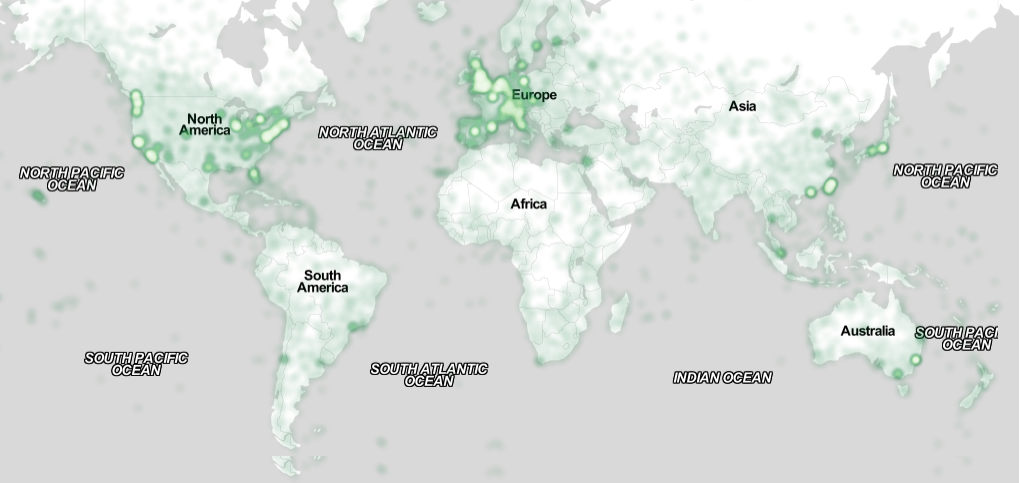
\includegraphics[width=1.75\columnwidth]{figures/map}
  \caption{In this image, the map maximizes use of space. You can make
    figures as wide as you need, up to a maximum of the full width of
    both columns. Note that \LaTeX\ tends to render large figures on a
    dedicated page. Image: \ccbynd~ayman on
    Flickr.}~\label{fig:figure2}
\end{figure*}




\begin{itemize}
\item Write in a straightforward style.
\item Try to avoid long or complex sentence structures.
\item Briefly define or explain all technical terms that may be
  unfamiliar to readers.
\item Explain all acronyms the first time they are used in your
  text---e.g., ``Digital Signal Processing (DSP)''.
\item Explain local references (e.g., not everyone knows all city
  names in a particular country).
\item Explain ``insider'' comments. Ensure that your whole audience
  understands any reference whose meaning you do not describe (e.g.,
  do not assume that everyone has used a Macintosh or a particular
  application).
\end{itemize}

following five steps:
\begin{enumerate}
\item Add alternative text to all figures
\item Mark table headings
\item Add tags to the PDF
\item Verify the default language
\item Set the tab order to ``Use Document Structure''
\end{enumerate}



\section{Acknowledgments}

Sample text: We thank all the volunteers, and all publications support
and staff, who wrote and provided helpful comments on previous
versions of this document. Authors 1, 2, and 3 gratefully acknowledge
the grant from NSF (\#1234--2012--ABC). \textit{This whole paragraph is
  just an example.}


\balance{}


% REFERENCES FORMAT
% References must be the same font size as other body text.
\bibliographystyle{SIGCHI-Reference-Format}
\bibliography{sample}

\end{document}

%%% Local Variables:
%%% mode: latex
%%% TeX-master: t
%%% End:
